\usepackage{upquote}

\section{Task 1 -- RQ1: Methodology \& Results}
\label{sec:rq1-methods}

\textbf{RQ1:} How do (selected) LLMs perform on cross-domain Text-to-SQL?


\subsection{Models}
\label{sec:models}

We compare two decoder-only LLMs from the same model family at different scales (Qwen3-0.6B and Qwen3-4B) against one reasoning LLM, so that the comparison isolates the effect of scale within a fixed family from the effect of an explicit reasoning trace, as much as a 3-model study can. All three are accessed as local inference over their bf16 Huggingface checkpoints on 1x NVIDIA GeForce RTX 4090 GPU (no API-based models), so that inference parameters are fully under our control (see \ref{sec:inference-settings}).

\begin{table}[H]
\centering
\footnotesize
\caption{Models compared in RQ1.}
\label{tab:models}
\resizebox{\textwidth}{!}{%
\begin{tabular}{llllll}
\toprule
Model & Category & Parameters & Quantization & Access & Thinking mode \\
\midrule
Qwen3-0.6B (Qwen Team, 2025) & Decoder-only & 0.6B & bf16 (none beyond release precision) & Local, Huggingface checkpoint & Disabled \\
Qwen3-4B (Qwen Team, 2025) & Decoder-only & 4B & bf16 (none beyond release precision) & Local, Huggingface checkpoint & Disabled \\
DeepSeek-R1-Distill-Qwen-1.5B (DeepSeek-AI, 2025) & Reasoning & 1.5B & bf16 (none beyond release precision) & Local, Huggingface checkpoint & Always on (no disable option) \\
\bottomrule
\end{tabular}}
\end{table}

All three are dense (non-MoE) models, so no distinction between total and active parameters applies.

\subsection{Evaluation Data}
\label{sec:eval-data}

We use all 1034 examples in the Spider (Yu et al., 2018) development split, with no subsampling and therefore no sampling seed to report; every example is included, so the per-database counts below and the per-database results tables (\hyperref[tab:db-execution]{Table 5} and \hyperref[tab:db-exact]{Table 6}) enumerate exactly which examples are used. To evaluate cross-domain performance, we additionally report results separately for each of the 20 databases in the Spider dev set: world\_1 (120 problems), car\_1 (92), cre\_Doc\_Template\_Mgt (84), dog\_kennels (82), flight\_2 (80), student\_transcripts\_tracking (78), wta\_1 (62), tvshow (62), network\_1 (56), concert\_singer (45), pets\_1 (42), poker\_player (40), orchestra (40), employee\_hire\_evaluation (38), course\_teach (30), singer (30), museum\_visit (18), battle\_death (16), voter\_1 (15), and real\_estate\_properties (4).

We also use the Spider Hardness Criteria, where queries are assigned difficulties based on the number of SQL components, selections, and conditions, so that queries that contain more SQL keywords are considered harder (figure~\ref{fig:hardness-levels} shows an example of each level).

\begin{figure}[H]
\centering
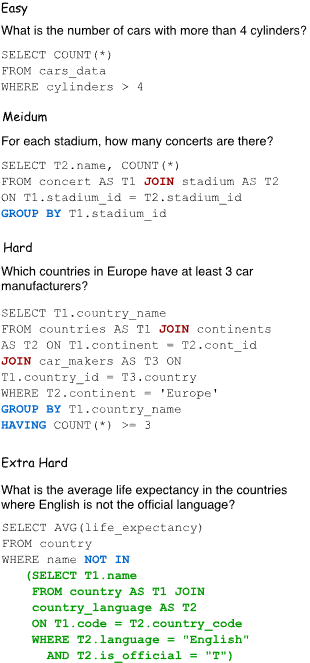
\includegraphics[width=0.35\textwidth]{image.png}
\caption{SQL query examples in 4 hardness levels. Credit: Spider (Yu et al., 2018)}
\label{fig:hardness-levels}
\end{figure}

\subsection{Prompting and Input}
\label{sec:prompting}

Each model receives three pieces of information in a single zero-shot user turn: a system instruction explaining its role as a Text-to-SQL generator, the database schema (Table names, column names, primary keys, and foreign-key relationships, with no example rows), and the natural-language question. No few-shot examples are provided, so that the experiment measures each model's ability to generate SQL from instructions and schema information alone, without the confound of examples steering its output style. The prompt template is identical across all three models, so that differences in performance can be attributed to the models rather than to differences in prompting.

\textbf{Prompt template:}
\begin{verbatim}
Given the following SQLite database schema, write a SQL query that answers
the question.

{schema}

Question: {question}

Respond with only the SQL query in a ```sql code block.
\end{verbatim}

See \hyperref[sec:appendix1]{Appendix 1} for a worked example: a full schema, a question, and the resulting filled prompt.

\subsection{SQL Extraction}
\label{sec:sql-extraction}

For each sample, we decode the model's generated tokens into text using the model-specific tokenizer, and check for the presence of a \texttt{</think>} token. If \texttt{</think>} was generated, we take all text generated before \texttt{</think>} as the reasoning trace and all text to the right as the output SQL; DeepSeek-R1-Distill-Qwen-1.5B is the only model of the three that can emit this token. The SQL is then extracted from the first \texttt{```sql} code block in that remaining text. The extracted SQL is passed to the evaluation script as-is. Outputs that cannot be extracted or parsed are counted as incorrect on every metric rather than excluded from the evaluation, as unusable output is a task failure (see \ref{sec:evaluation-metrics} and \ref{sec:invalid-outputs}).

\subsection{Inference Settings}
\label{sec:inference-settings}

All models are evaluated using the same decoding configuration: greedy decoding (temperature and top-p are not applicable) for consistent, reproducible results between runs. The maximum output length differs by model: 256 tokens for Qwen3-0.6B, and 4096 tokens for both Qwen3-4B and DeepSeek-R1-Distill-Qwen-1.5B. For DeepSeek, the larger budget is needed because its output also has to contain a full reasoning trace rather than only the SQL query; Qwen3-4B is given the same, larger budget as DeepSeek so that a tighter token limit can be ruled out as the reason for any difference between them on invalid-output rate (\ref{sec:invalid-outputs}) or inference time (\ref{sec:efficiency}). Qwen3-0.6B and Qwen3-4B are both run with thinking mode off (both support it). DeepSeek-R1-Distill-Qwen-1.5B always produces a reasoning trace and has no documented way to disable thinking mode, so it is evaluated as the reasoning condition against the two non-reasoning Qwen3 models. All inference runs on the same 1x RTX 4090 GPU described in \ref{sec:models}, with batch size 128.

\subsection{Evaluation}
\label{sec:evaluation-metrics}

We evaluate the output using the same metrics as the Spider paper (Yu et al., 2018). These are:

\begin{enumerate}
\item Component Matching
    \begin{itemize}
        \item For each of the following components:
        \begin{itemize}
            \item SELECT
            \item WHERE
            \item GROUP BY
            \item ORDER BY
            \item KEYWORDS (including all SQL keywords without column names and operators)
        \end{itemize}
        \item Decompose each component in the prediction and ground truth as bags of several sub-components and check whether or not these two sets of components match completely.
        \item Checks accuracy, recall, and F1
    \end{itemize}
\item Exact Matching Accuracy
    \begin{itemize}
        \item We measure whether the generated query as a whole is equivalent to the golden query (AKA ground truth query)
        \item The generated query is correct only if all components are correct
        \item Checks only accuracy
    \end{itemize}
\item Execution Accuracy
    \begin{itemize}
        \item A list of gold values for each question is given
        \item We measure how many gold values the generated query extracts when executed
        \item Checks only accuracy
    \end{itemize}
\end{enumerate}

If output is invalid or unparsable, then it fails exact matching and execution accuracy. Results~\ref{sec:invalid-outputs} reports how often this happens for each model.

\section{RQ1: Results}
\label{sec:rq1-results}

\subsection{Overall Model Performance}
\label{sec:overall-performance}

Below we report how Qwen3-0.6B, Qwen3-4B, and DeepSeek-R1-Distill-Qwen-1.5B perform on the Spider benchmark across all 3 metrics (Component Matching, Exact Matching Accuracy, Execution Accuracy). We calculate the values per problem difficulty as well as overall, and display them in the below tables.

\begin{table}[H]
\centering
\footnotesize
\caption{Overall performance summary, aggregated across all difficulties (all 1034 problems). Component matching is accuracy / recall / F1 (macro-averaged, see the note on Table~\ref{tab:difficulty-component} in \ref{sec:rq1-interpretation}). Per-difficulty breakdowns are in Tables~\ref{tab:difficulty-component}--\ref{tab:difficulty-execution}.}
\label{tab:overall-performance}
\resizebox{\textwidth}{!}{%
\begin{tabular}{lllccc}
\toprule
Model & Parameters & Category & Component matching & Exact matching & Execution accuracy \\
\midrule
Qwen3-0.6B & 0.6B & Decoder-only & 0.628 / 0.209 / 0.314 & 0.099 & 0.209 \\
Qwen3-4B & 4B & Decoder-only & 0.797 / 0.306 / 0.442 & 0.256 & 0.353 \\
DeepSeek-R1-Distill-Qwen-1.5B & 1.5B & Reasoning & 0.661 / 0.174 / 0.275 & 0.085 & 0.121 \\
\bottomrule
\end{tabular}}
\end{table}

All models are evaluated zero-shot with the same prompt on the 20 databases of the Spider dev set. Aggregated across all difficulties and databases, every model is still far from solving the task: execution accuracy ranges from 0.121 (DeepSeek) to 0.353 (Qwen3-4B) and exact matching accuracy from 0.085 (DeepSeek) to 0.256 (Qwen3-4B). Execution accuracy is higher than exact matching accuracy for all three models (for example 0.353 vs.\ 0.256 for Qwen3-4B), which suggests that at least some of the queries that return the correct result are written differently from the gold SQL (see Section \ref{sec:rq1-interpretation} for more on this relationship). Of the three models, Qwen3-4B is now the best on almost every metric, database, and difficulty level; Section \ref{sec:by-database} and Section \ref{sec:rq1-interpretation} quantify how consistently. Table ~\ref{tab:inference-time} reports the efficiency side of this comparison: inference time per example.

\subsection{Performance by Query Difficulty}
\label{sec:by-difficulty}

\begin{table}[H]
\centering
\footnotesize
\caption{Component matching (accuracy / recall / F1) by difficulty.}
\label{tab:difficulty-component}
\begin{tabular}{lcc}
\toprule
Model & easy & medium \\
\midrule
Problems (n) & 248 & 446 \\
Qwen3-0.6B & 0.675 / 0.308 / 0.423 & 0.582 / 0.235 / 0.334 \\
Qwen3-4B & 0.838 / 0.574 / 0.681 & 0.670 / 0.306 / 0.420 \\
DeepSeek-R1-Distill-Qwen-1.5B & 0.566 / 0.288 / 0.382 & 0.642 / 0.185 / 0.287 \\
\bottomrule
\end{tabular}

\vspace{0.5em}

\begin{tabular}{lccc}
\toprule
Model & hard & extra & all \\
\midrule
Problems (n) & 174 & 166 & 1034 \\
Qwen3-0.6B & 0.540 / 0.141 / 0.223 & 0.578 / 0.160 / 0.250 & 0.628 / 0.209 / 0.314 \\
Qwen3-4B & 0.796 / 0.262 / 0.394 & 0.485 / 0.150 / 0.229 & 0.797 / 0.306 / 0.442 \\
DeepSeek-R1-Distill-Qwen-1.5B & 0.543 / 0.113 / 0.187 & 0.389 / 0.104 / 0.164 & 0.661 / 0.174 / 0.275 \\
\bottomrule
\end{tabular}
\end{table}

\begin{table}[H]
\centering
\footnotesize
\caption{Exact matching accuracy by difficulty.}
\label{tab:difficulty-exact}
\begin{tabular}{lccccc}
\toprule
Model & easy & medium & hard & extra & all \\
\midrule
Problems (n) & 248 & 446 & 174 & 166 & 1034 \\
Qwen3-0.6B & 0.157 & 0.137 & 0.006 & 0.006 & 0.099 \\
Qwen3-4B & 0.508 & 0.262 & 0.115 & 0.012 & 0.256 \\
DeepSeek-R1-Distill-Qwen-1.5B & 0.214 & 0.078 & 0.000 & 0.000 & 0.085 \\
\bottomrule
\end{tabular}
\end{table}

\begin{table}[H]
\centering
\footnotesize
\caption{Execution accuracy by difficulty.}
\label{tab:difficulty-execution}
\begin{tabular}{lccccc}
\toprule
Model & easy & medium & hard & extra & all \\
\midrule
Problems (n) & 248 & 446 & 174 & 166 & 1034 \\
Qwen3-0.6B & 0.210 & 0.276 & 0.126 & 0.114 & 0.209 \\
Qwen3-4B & 0.565 & 0.345 & 0.276 & 0.139 & 0.353 \\
DeepSeek-R1-Distill-Qwen-1.5B & 0.258 & 0.128 & 0.017 & 0.006 & 0.121 \\
\bottomrule
\end{tabular}
\end{table}

We break every metric down by the Spider Hardness Criteria (\ref{sec:eval-data}), since aggregate numbers alone would hide whether a model's advantage holds up as queries get harder.

Performance decreases with difficulty for every model, but the decrease is steepest for Qwen3-0.6B and DeepSeek: their exact matching and execution accuracy are both at most 0.006 and 0.126 respectively on hard and extra problems, down from as high as 0.210-0.258 (easy execution) on the easiest problems (Table~\ref{tab:difficulty-exact} and Table~\ref{tab:difficulty-execution}). Qwen3-4B degrades on the same relative scale but from a much higher starting point, from 0.508 easy exact matching / 0.565 easy execution accuracy down to 0.012 extra exact matching / 0.139 extra execution accuracy. Despite the degradation, it remains the best of the three models at every single difficulty level on both metrics (Tables~\ref{tab:difficulty-exact}--\ref{tab:difficulty-execution}).

\subsection{Performance by Database}
\label{sec:by-database}

We also break execution and exact matching accuracy down by each of the 20 Spider dev databases. Qwen3-4B has the highest execution accuracy on 17 of the 20 databases outright (plus a tie on one more) and the highest exact matching accuracy on 18 of 20, while DeepSeek-R1-Distill-Qwen-1.5B is never highest on either metric; Qwen3-0.6B wins outright only on orchestra and battle\_death. Databases with few problems (real\_estate\_properties with n=4, voter\_1 with n=15, battle\_death with n=16, and museum\_visit with n=18) are too small to rank the models reliably, since a single problem changes a score by 6 to 25 percentage points. Execution accuracy ranges from 0.10 (course\_teach) to 0.53 (singer) for Qwen3-0.6B, from 0.19 (battle\_death) to 0.60 (singer) for Qwen3-4B, and from 0.00 (concert\_singer) to 0.27 (singer and voter\_1) for DeepSeek-R1-Distill-Qwen-1.5B (\hyperref[tab:db-execution]{Table 5}). 


\begin{table}[H]
\centering
\footnotesize
\caption{Execution accuracy by database (domain).}
\begin{tabular}{lcccc}
\toprule
Database & Problems (n) & Qwen3-0.6B & Qwen3-4B & DeepSeek-R1-Distill-Qwen-1.5B \\
\midrule
world\_1 & 120 & 0.183 & 0.242 & 0.108 \\
car\_1 & 92 & 0.109 & 0.315 & 0.054 \\
cre\_Doc\_Template\_Mgt & 84 & 0.202 & 0.405 & 0.071 \\
dog\_kennels & 82 & 0.159 & 0.293 & 0.085 \\
flight\_2 & 80 & 0.263 & 0.500 & 0.250 \\
student\_transcripts\_tracking & 78 & 0.128 & 0.321 & 0.064 \\
wta\_1 & 62 & 0.161 & 0.290 & 0.129 \\
tvshow & 62 & 0.339 & 0.435 & 0.129 \\
network\_1 & 56 & 0.286 & 0.375 & 0.179 \\
concert\_singer & 45 & 0.111 & 0.289 & 0.000 \\
pets\_1 & 42 & 0.167 & 0.286 & 0.071 \\
poker\_player & 40 & 0.250 & 0.550 & 0.225 \\
orchestra & 40 & 0.350 & 0.250 & 0.100 \\
employee\_hire\_evaluation & 38 & 0.105 & 0.211 & 0.132 \\
course\_teach & 30 & 0.100 & 0.500 & 0.100 \\
singer & 30 & 0.533 & 0.600 & 0.267 \\
museum\_visit & 18 & 0.278 & 0.500 & 0.222 \\
battle\_death & 16 & 0.375 & 0.188 & 0.188 \\
voter\_1 & 15 & 0.267 & 0.400 & 0.267 \\
real\_estate\_properties & 4 & 0.500 & 0.500 & 0.000 \\
\bottomrule
\label{tab:exec-acc-rq1-by-database}
\end{tabular}
\end{table}


The pattern on exact matching accuracy is just as one-sided (\hyperref[tab:db-exact]{Table 6}): Qwen3-4B is highest on 18 of 20 databases, ties Qwen3-0.6B on orchestra, and loses only on battle\_death; DeepSeek's exact matching accuracy is never the highest of the three, coming closest on flight\_2 (0.200 vs.\ Qwen3-4B's 0.350 and Qwen3-0.6B's 0.075). The full per-database tables and discussion are in \hyperref[sec:appendix2]{Appendix 2}.

\subsection{Analysis of Invalid and Unparseable Outputs}
\label{sec:invalid-outputs}

We also count how often each model's output cannot be used as SQL at all: it either never produces a usable query within the token budget (\ref{sec:inference-settings}) or is truncated before finishing one. Per \ref{sec:evaluation-metrics}, these count as failures on every metric rather than being excluded, and this is a direct measure of how reliably each model follows the ``respond with only a SQL query'' instruction, independent of whether the SQL it does produce is correct. Qwen3-0.6B's invalid rate is 2.2\%, Qwen3-4B's is 0.0\%, and DeepSeek-R1-Distill-Qwen-1.5B's is 9.7\%, about 4x higher than Qwen3-0.6B's despite having the same 4096-token budget as Qwen3-4B (\ref{sec:inference-settings}), i.e. a larger token budget did not cause Qwen3-4B to run on or produce unusable output the way it does for DeepSeek. Section \ref{sec:rq1-interpretation} breaks DeepSeek's failures down further by difficulty and by why the generation failed (see Tables~\ref{tab:deepseek-outcome}--\ref{tab:deepseek-unfinished-by-difficulty}).


\begin{table}[H]
\centering
\footnotesize
\caption{DeepSeek-R1-Distill-Qwen-1.5B by generation outcome. ``Cut'' means the generation reached the 4096-token limit.}
\label{tab:deepseek-outcome}
\begin{tabular}{lccccc}
\toprule
Outcome & Problems (n) & Share & Avg.\ tokens & Exact match & Component F1 \\
\midrule
Finished with SQL & 934 & 90.3\% & 512 & 0.094 & 0.286 \\
Finished, no usable SQL & 2 & 0.2\% & 284 & 0.000 & 0.100 \\
Cut while answering (after \texttt{</think>}) & 13 & 1.3\% & 4096 & 0.000 & 0.096 \\
Cut while thinking (no \texttt{</think>}) & 85 & 8.2\% & 4096 & 0.000 & 0.093 \\
All & 1034 & 100\% & 851 & 0.085 & 0.275 \\
\bottomrule
\end{tabular}
\end{table}

\begin{table}[H]
\centering
\footnotesize
\caption{The same 934 questions that DeepSeek finished, for all three models.}
\label{tab:deepseek-finished-934}
\begin{tabular}{lcc}
\toprule
Model & Exact match & Component F1 \\
\midrule
DeepSeek-R1-Distill-Qwen-1.5B & 0.094 & 0.286 \\
Qwen3-0.6B & 0.103 & 0.317 \\
Qwen3-4B & 0.257 & 0.440 \\
\bottomrule
\end{tabular}
\end{table}

\begin{table}[H]
\centering
\footnotesize
\caption{Share of Deepseek generations that are infinite self-repetition loops. We check self-repetition using compression ratio: a text that repeats itself compresses well, so a low compression ratio of the last 3000 characters indicates a loop. In testing, we found generations with compression ratios <0.15 infinitely self-looped.}
\label{tab:deepseek-repetition}
\begin{tabular}{lcccc}
\toprule
Generations & n & Median compression ratio & Ratio $<$ 0.15 & Last 150 characters repeat 3 or more times \\
\midrule
Cut off & 98 & 0.095 & 95.9\% & 96.9\% \\
Finished & 936 & 0.418 & 0.0\% & 0.2\% \\
\bottomrule
\end{tabular}
\end{table}

\begin{table}[H]
\centering
\footnotesize
\caption{Share of DeepSeek generations that did not finish with SQL, by difficulty.}
\label{tab:deepseek-unfinished-by-difficulty}
\begin{tabular}{lccccc}
\toprule
 & easy & medium & hard & extra & all \\
\midrule
Problems (n) & 248 & 446 & 174 & 166 & 1034 \\
Not finished with SQL (n) & 15 & 33 & 25 & 27 & 100 \\
Share & 6.0\% & 7.4\% & 14.4\% & 16.3\% & 9.7\% \\
\bottomrule
\end{tabular}
\end{table}

\subsection{Efficiency Measures}
\label{sec:efficiency}

\begin{table}[H]
\centering
\footnotesize
\caption{Output tokens per example.}
\label{tab:tokens-per-example}
\begin{tabular}{lccccc}
\toprule
Model & easy & medium & hard & extra & all \\
\midrule
Qwen3-0.6B & 27.5 & 44.7 & 53.7 & 69.9 & 46.1 \\
Qwen3-4B & 23.6 & 37.3 & 46.2 & 59.0 & 39.0 \\
DeepSeek-R1-Distill-Qwen-1.5B & 610.8 & 768.4 & 1096.0 & 1176.9 & 851.3 \\
\bottomrule
\end{tabular}
\end{table}

Inference time is measured from the start of generation to the complete batch output, per batch of 128 examples, with each batch's wall time divided evenly across its 128 examples to get the per-example figure, excluding tokenization, model loading, and warm-up.

\begin{table}[H]
\centering
\footnotesize
\caption{Inference time.}
\label{tab:inference-time}
\begin{tabular}{lcc}
\toprule
Model & Total wall time (s) & Avg.\ time per example (s) \\
\midrule
Qwen3-0.6B & 123.9 & 0.120 \\
Qwen3-4B & 109.1 & 0.106 \\
DeepSeek-R1-Distill-Qwen-1.5B & 3059.8 & 2.959 \\
\bottomrule
\end{tabular}
\end{table}

DeepSeek is about 25x slower per example than Qwen3-0.6B and 28x slower than Qwen3-4B, consistent with its much higher average token count (Table~\ref{tab:tokens-per-example}). Qwen3-4B, despite having about 7x as many parameters as Qwen3-0.6B, is marginally faster per example (0.106s vs.\ 0.120s), consistent with it generating fewer tokens on average (39.0 vs.\ 46.1, Table~\ref{tab:tokens-per-example}) despite having the same 16x larger token budget as DeepSeek (\ref{sec:inference-settings}).


\section{RQ1: Interpretation and Answer}
\label{sec:rq1-interpretation}

\textbf{RQ1:} How do (selected) LLMs perform on cross-domain Text-to-SQL?

\vspace{10px}

All three models are still far from solving the task in this zero-shot setting: exact matching accuracy ranges from 0.085 to 0.256 and execution accuracy from 0.121 to 0.353 (Table~\ref{tab:overall-performance}). Difficulty and database effects are discussed in \ref{sec:by-difficulty} and \ref{sec:by-database}; here we interpret the effects of model size and reasoning architecture and the exact-match/execution-accuracy relationship, and state the answer to RQ1 as three findings.

\subsection{First, within the Qwen family, scale is a strong and almost uniform predictor of performance, but an intermediate-size reasoning model from the DeepSeek family still loses to the smallest model in the Qwen family.}
\label{sec:rq1-finding-scale}

Aggregated across all difficulties, Qwen3-4B has the best component matching (0.797 accuracy / 0.306 recall / 0.442 F1), exact matching (0.256 ), and execution accuracy (0.353) of the three (Table~\ref{tab:overall-performance}), and it beats Qwen3-0.6B on exact matching and execution accuracy at every individual difficulty level, including hard (0.115 vs.\ 0.006) and extra (0.012 vs.\ 0.006), where the smaller model solves almost nothing (Tables~\ref{tab:difficulty-exact}--\ref{tab:difficulty-execution}). This effect is large and holds at every difficulty level. The one exception is component matching on extra-hard problems, where Qwen3-0.6B's accuracy, recall, and F1 (0.578 / 0.160 / 0.250) are all slightly higher than Qwen3-4B's (0.485 / 0.150 / 0.229), the only point in the RQ1 results where the smaller Qwen3 model wins outright (Table~\ref{tab:difficulty-component}). DeepSeek-R1-Distill-Qwen-1.5B sits between the two Qwen3 models in parameter count (1.5B) and is the only one that reasons, yet it is the lowest of the three on every aggregate metric (0.275 component F1, 0.085 exact matching, 0.121 execution accuracy) except its own component-matching accuracy (0.661 vs.\ 0.628 for Qwen3-0.6B). Thus, scale predicts performance well within a family, but does not transfer across the reasoning/non-reasoning boundary: having more parameters than Qwen3-0.6B did not help DeepSeek catch up to it.

\subsection{Second, the reasoning architecture itself, not parameter count, is the most likely driver of DeepSeek's low score.}
\label{sec:rq1-finding-reasoning}

Its invalid-output rate (9.7\%) is markedly higher than Qwen3-0.6B's (2.2\%) and Qwen3-4B's (0.0\% in this run) (\ref{sec:invalid-outputs}). In Tables~\ref{tab:deepseek-outcome}--\ref{tab:deepseek-unfinished-by-difficulty}, 100 of 1034 generations (9.7\%) end without usable SQL. 85 never leave the reasoning phase, 13 are cut while writing the answer, and 2 finish without SQL. The number of unusable SQL generations also grows with difficulty, from 6.0\% on easy to 16.3\% on extra problems. These are not cases of long productive reasoning either: 95.9\% of the cut-off generations are highly self-repetitive (compression ratio below 0.15, median compression ratio 0.095, vs.\ 0.418 for finished generations), rewriting the same query and repeating phrases like ``So the final query is:'' without converging. Finishing does not make it better either: on the 934 questions DeepSeek does finish, its exact matching (0.094) and component F1 (0.286) are still below Qwen3-0.6B's on the same questions (0.103 / 0.317) and far below Qwen3-4B's (0.257 / 0.440), despite generating 512 tokens per question on average there, against 46 and 39 tokens overall for Qwen3-0.6B and Qwen3-4B (about 11x and 13x fewer). This extra length also costs time: DeepSeek is 25-28x slower per example than either Qwen3 model (\ref{sec:efficiency}). The reasoning trace mostly lengthens the output and sometimes never terminates, without improving the SQL when it does, and size alone is not the explanation, since Qwen3-4B is both bigger than DeepSeek and the best model in the comparison. This does not fully isolate reasoning from DeepSeek's other differences from the two Qwen3 models, such as distillation (see Limitations).

\subsection{Third, query difficulty has a substantial, consistent effect on every model, including the best one.}
\label{sec:rq1-finding-difficulty}

Exact matching and execution accuracy both fall sharply from easy to extra-hard problems for all three models (\ref{sec:by-difficulty}). Qwen3-4B's drop is from a much higher base (0.508 to 0.012 exact matching, 0.565 to 0.139 execution accuracy) and it remains the best model at every difficulty level on both metrics, but the drop itself is just as steep in relative terms as for the other two models, and the hardest problems remain largely unsolved even for it.

\subsection{Exact Match vs.\ Execution Accuracy}
\label{sec:rq1-exact-vs-execution}

For all three models, execution accuracy aggregated across all difficulties exceeds exact matching accuracy (Table~\ref{tab:overall-performance}): 0.209 vs.\ 0.099 for Qwen3-0.6B, 0.353 vs.\ 0.256 for Qwen3-4B, and 0.121 vs.\ 0.085 for DeepSeek. Since exact matching requires every SQL component to match the gold query while execution accuracy only requires the same result set, this gap indicates each model writes some queries that are valid and correct but phrased differently from the gold SQL (e.g.\ a different but equivalent join order, or an explicit column list where the gold query uses \texttt{SELECT *}). The gap is widest for Qwen3-0.6B (11.0 points), close behind for Qwen3-4B (9.7 points), and narrowest for DeepSeek (3.6 points); DeepSeek's narrower gap reflects it producing fewer alternative-but-valid queries. Qwen3-4B's gap is almost as wide as Qwen3-0.6B's despite much higher absolute accuracy, so scaling up within the Qwen3 family raises both exact matching accuracy and execution accuracy together rather than closing the gap between them.

\subsection{Limitations}
\label{sec:rq1-limitations}

Our working hypothesis is that Text-to-SQL at this scale does not benefit from an explicit reasoning trace, and that a non-reasoning model is sufficient, with performance instead scaling with parameter count within a fixed model family. The results are consistent with this hypothesis. However, they do not establish that Text-to-SQL is too simple for reasoning models in general due to several factors:

\begin{itemize}
\item \textbf{Model differences beyond reasoning.} Qwen3-0.6B and Qwen3-4B share a model family, isolating the effect of scale between them, but DeepSeek differs from both in family, size, and pretraining/post-training, not only in whether it reasons; it is also a distilled model, so the effect of reasoning cannot be fully separated from distillation quality.
\item \textbf{Aggregated component matching.} The component matching figures in Table~\ref{tab:difficulty-component} (and in Table~\ref{tab:overall-performance}) are our own macro-average (mean of the 10 per-component accuracy and recall scores, with F1 computed from these two means), not a number reported by Spider.
\end{itemize}

Overall, in this zero-shot, cross-domain setting, a larger non-reasoning decoder-only model (Qwen3-4B, 4B) clearly outperforms both a same-family model at under a sixth its size (Qwen3-0.6B) and a reasoning model of intermediate size from a different family (DeepSeek-R1-Distill-Qwen-1.5B, 1.5B), while also being faster per example than either. None of the three models solve more than half of even the easiest problems or more than a small fraction of hard or extra-hard queries. This answers RQ1 for the three models evaluated.